\documentclass[sigconf]{acmart}
\settopmatter{printacmref=false}
\setcopyright{none}
\renewcommand\footnotetextcopyrightpermission[1]{}
\acmConference[SIGMOD-Companion '27]{Companion of the 2027 International Conference on Management of Data}{June 13--18, 2027}{Huntington Beach, CA, USA}
\usepackage{booktabs}
\usepackage{amsmath}
\usepackage{algorithm}
\usepackage{algpseudocode}
\usepackage{listings}
\lstset{basicstyle=\ttfamily\scriptsize,columns=fullflexible,keepspaces=true,frame=tb,framerule=0.4pt,
  keywordstyle=\bfseries,language=SQL,morekeywords={WITH,OVER,PARTITION,LEAD,ROWS,UNBOUNDED,PRECEDING,USING},
  aboveskip=4pt,belowskip=2pt,xleftmargin=2pt}
\newcommand{\autos}{\textsc{auto\_suspend}}
\newcommand{\yes}{\checkmark}
\newcommand{\no}{$\times$}

\emergencystretch=1.5em
\begin{document}
\title{Who Pays for Idle? Fair Chargeback for Shared Cloud Data Warehouses}

% AUTHOR LIST IS FROZEN AT SUBMISSION (SIGMOD industrial rules) -- confirm names, order, affiliations before Nov 24.
\author{Khadarvali Shaik}
\affiliation{\institution{[Affiliation -- non-academic]}\city{Richmond}\state{VA}\country{USA}}
\email{khadarvali.shaik@ieee.org}

\begin{abstract}
When several teams share one cloud data warehouse, someone has to turn a single invoice into per-team charges. Warehouses
bill per second while they run, with a minimum on every resume and an idle tail until auto-suspend, but per-query
attribution assigns only the time queries spend executing. On three months of per-user query history from the 94 shared
instances in Amazon's Redset trace, execution-time attribution leaves a median 31--56\% of the bill unassigned, depending
on the auto-suspend setting; in a two-hour live run of short queries on Snowflake, the platform's own attribution left 88--93\%
unassigned. Teams split this remainder with ad hoc rules. We show that the common rules are unfair in ways a finance team
would notice: proportional splitting charges 12--17\% of team-months more than a private warehouse would cost them (a median
33--44\% more), equal splitting overcharges 33--44\%, and when one team adds a few scattered queries, proportional and
marginal-cost splitting raise another team's charge in 41--68\% and 26--50\% of cases. We model chargeback as a cost-sharing game defined by the billing rules and prove that,
when auto-suspend is at least the 60-second resume minimum, the game is a coverage game: its Shapley value is in the core,
never penalises bystanders, and is computed exactly in $O(m\log m)$ for $m$ queries by splitting each billed second among
the teams that keep it running. The rule fits in one SQL query. Across 25,856 coalition checks and 14,192 growth cases
per setting, it never charges a team or group above its standalone cost at observed timing and never raises a bystander's
charge; if teams ran 10\% faster alone, it would exceed that cost for 3--9\% of team-months by a median 0.4--2\%, against
9--40\% of team-months for the common rules. Our engine
reproduces the running time in Snowflake's warehouse events to within 1.2\%; code, results and the pre-registration are public.
\end{abstract}

\begin{CCSXML}
<ccs2012><concept><concept_id>10002951.10002952</concept_id><concept_desc>Information systems~Data management systems</concept_desc><concept_significance>500</concept_significance></concept></ccs2012>
\end{CCSXML}
\ccsdesc[500]{Information systems~Data management systems}
\keywords{cloud data warehouse, chargeback, cost attribution, Shapley value, auto-suspend, FinOps}

\maketitle

\section{Introduction}
Shared warehouses are cheaper than one warehouse per team: idle tails and resume minimums are paid once instead of many
times. The saving creates a new problem. The cloud provider sends one invoice per warehouse, and the platform team that runs
it must decide how much each consuming team pays. In practice this \emph{chargeback} (or, when no money moves,
\emph{showback}) drives budgets, prompts disputes, and shapes behaviour: teams that believe they are overcharged ask for a
private warehouse, which costs the organisation more, and teams that believe they ride free have no reason to change.
In the author's experience operating a shared Snowflake platform for many engineering teams, chargeback disputes follow
a pattern. A team issuing short scheduled queries is charged little under execution-time attribution yet keeps the
warehouse awake all day. A team with long batch jobs pays most under proportional splitting and asks for a private
warehouse. Each new tenant changes everyone else's charge. Finance wants a split that adds up to the invoice and that
teams accept as fair.

Cloud data warehouses now expose per-query cost attribution. Snowflake's
\texttt{QUERY\_\allowbreak ATTRIBUTION\_\allowbreak HISTORY}, for example, assigns warehouse credits to queries in
proportion to their resource use while they run, but explicitly excludes idle time~\cite{sf-attribution}. Idle time is not a
rounding error. A warehouse is billed per second from resume until it suspends, with a 60-second minimum on each resume, and it stays
up for \autos{} seconds after the last query ends~\cite{sf-warehouses,sf-create}. For bursty, interactive workloads most of
the bill is this tail. What is left after attribution is split by rules of thumb: in proportion to attributed usage,
equally, or by some marginal-cost calculation. None of them was designed for the billing contract it is applied to.

This paper asks whether those rules are fair, and what a fair rule looks like that a platform team can run on a real fleet.
We make five contributions.
\begin{itemize}
\item \textbf{Measurement.} On Redset~\cite{redset}, three months of per-user query history from 94 shared Amazon Redshift
instances (247.8 million queries), replayed under per-second warehouse billing, execution-time attribution leaves a median
31\% (60\,s auto-suspend) to 56\% (600\,s, Snowflake's default) of the bill unassigned (Section~\ref{sec:e2}). In a live run
on Snowflake with short queries, the platform's own attribution left 88--93\% unassigned.
\item \textbf{Fairness properties and failures.} We state three properties a chargeback should satisfy---full recovery, no
team or group charged above its standalone cost, no bystander penalised for another team's growth---and show, in theory and
on the fleet, how the common rules violate them (Sections~\ref{sec:rules},~\ref{sec:e3}).
\item \textbf{A tractable fair rule.} We prove that warehouse billing with \autos{} $\ge$ 60\,s is a coverage game, so its
Shapley value is in the core, is monotone for bystanders, and is computable exactly by one sweep over query intervals
(Section~\ref{sec:model}). We also show where the result stops: below 60\,s the game need not be concave, and labels matter. The game theory is
classical---coverage games and their Shapley values are well understood~\cite{shapley71,littlechild73}---and our contribution
is to show that a real billing contract is such a game, where it stops being one, and what that means in practice.
\item \textbf{An engine, validated.} The engine reproduces Snowflake's actual running periods to within 1.2\%, allocates the
full metered invoice, and runs in about a second per million queries as a single SQL statement in DuckDB
(Sections~\ref{sec:impl},~\ref{sec:e1}).
\item \textbf{Who pays more under a fair rule.} Shapley moves cost onto the teams whose short, scattered queries keep the
warehouse awake, and away from teams whose long queries already account for the time (Section~\ref{sec:who}).
\end{itemize}
The main fleet experiments were pre-registered before they were run, two deviations are disclosed (Section~\ref{sec:method}),
and exploratory results are marked as such. Code, results and the pre-registration are public (Section~\ref{sec:artifacts}).

\section{Background and Related Work}\label{sec:background}
\textbf{Warehouse billing.} A Snowflake virtual warehouse is a cluster of fixed size that consumes credits at a size-dependent
rate while it runs~\cite{snowflake16,sf-warehouses}. Billing is per second with a 60-second minimum each time the warehouse
starts; it suspends after \autos{} seconds without running queries (default 600\,s)~\cite{sf-create}. On our trial account
an X-Small Gen2 warehouse consumed 1.35 credits per hour of running time. The same structure---a running resource
billed by time, with a start-up minimum and an idle timeout---applies to other serverless and provisioned warehouses, which
is why we can replay Redshift workloads under it.

\textbf{Attribution and chargeback in practice.} Per-query attribution answers ``what did this query cost while it ran''; it
does not answer ``who should pay for the minutes nobody was running anything''. Snowflake's view is explicit that idle time
is excluded~\cite{sf-attribution}. The FinOps Foundation's framework treats showback as always required and chargeback
as a formal step whose handling of shared costs the FinOps team and finance must decide together~\cite{finops}; it does not
say how to split idle time. In practice the gap is filled with tags and proportional allocation of the remainder. We are not aware of a study that measures how large the remainder is
across a fleet, or whether the proportional rule is fair under the billing contract it is applied to.

\textbf{Cost sharing and the Shapley value.} Shapley's value~\cite{shapley53} is the unique allocation that is efficient,
symmetric, additive and gives nothing to a team that adds no cost; for concave (submodular) cost games it lies in the
core~\cite{shapley71}. It has been used for cloud and shared-system pricing before: to price shared indexes and views among
tenants of a data service~\cite{upadhyaya12}, to attribute a provider's peak-based electricity costs to
tenants~\cite{nasiriani16}, and to set fees for a shared computer centre modelled as a queue~\cite{mclean98}. Closed forms
exist for special games, such as the airport game~\cite{littlechild73}, where each player pays an equal share of every
runway segment it needs; our result is a time-axis analogue. Those works price a provider's costs to its customers. Our
setting is a customer's internal invoice under a concrete billing contract, evaluated on real fleet traces and validated
against real metering. Engine-side cost optimisation (e.g., automatic scaling in Redshift~\cite{rais24} and
cost-intelligent warehouses~\cite{costintel24}) decides how much compute to run; it does not split the resulting bill.
This paper takes the shared warehouse as given and asks only how its bill is divided, not which warehouses an organisation
should run.

\section{Billing as a Cost-Sharing Game}\label{sec:model}
Consider one warehouse of fixed size, auto-suspend $a$ seconds and resume minimum $\mu = 60$\,s, over one billing month.
A set $N$ of $n$ teams submits $m$ queries; query $q$ executes on $[s_q, e_q]$ and belongs to one team. For a coalition
$S \subseteq N$, the \emph{standalone cost} $c(S)$ is the billed seconds the warehouse would incur if only $S$'s queries ran,
with the same timing (assumption A1: removing teams does not change the remaining queries' timing); the warehouse suspends
exactly $a$ seconds after its last running query (A2). Credits are billed seconds times a size-dependent rate, so we work in
seconds throughout.

\begin{lemma}[Running periods]\label{lem:periods}
Let $R(S) = \bigcup_{q \in S} [s_q, e_q + a]$. Under A2, the warehouse's running periods under $S$ are exactly the connected
components of $R(S)$, and $c(S) = \sum_{C} \max(\mu, |C|)$ over those components.
\end{lemma}
\begin{proof}
Order $S$'s queries by start. The first query resumes the warehouse. Inductively, let the current period have latest
query end $E$. A query with $s_q \le E + a$ starts before the suspend at $E + a$, so it lies in the same component of $R(S)$
and moves the end to $\max(E, e_q)$; a query with $s_q > E + a$ starts after the suspend and opens a new component. The last
period ends at its latest end plus $a$. Each period is billed for its length, but at least $\mu$.
\end{proof}

\begin{theorem}[Coverage game]\label{thm:coverage}
If $a \ge \mu$, then $c(S) = \bigl|\bigcup_{i \in S} A_i\bigr|$ with $A_i = R(\{i\})$. Consequently:
(i) the Shapley value is
\[\phi_i \;=\; \int_{A_i} \frac{dx}{|N(x)|}, \qquad N(x) = \{\, j \in N : x \in A_j \,\};\]
(ii) $\phi$ is in the core: $\sum_{i \in S} \phi_i \le c(S)$ for every $S$, with equality for $S = N$;
(iii) $\phi$ is computable exactly in $O(m \log m)$ time.
\end{theorem}
\begin{proof}
Every component of $R(S)$ ends with a full tail of length $a \ge \mu$, so $|C| \ge \mu$ and the minimum never binds;
by Lemma~\ref{lem:periods}, $c(S) = |R(S)|$. Since $R(S)$ is a union over queries, $R(S) = \bigcup_{i\in S} R(\{i\})$.

(i) For a point $x$, let $u_x(S) = \mathbf{1}[S \cap N(x) \neq \emptyset]$. Then $c(S) = \int u_x(S)\,dx$. In $u_x$, every
team outside $N(x)$ is a null player and the members of $N(x)$ are symmetric, so the Shapley value of $u_x$ gives
$1/|N(x)|$ to each member of $N(x)$ and $0$ to the others. The Shapley value is linear in the game, and the integral is an
exact finite sum over the elementary segments defined below, on which $u_x$ is constant; hence (i).

(ii) A union-measure function is submodular: for $S \subseteq T$ and $i \notin T$,
$c(S \cup \{i\}) - c(S) = |A_i \setminus R(S)| \ge |A_i \setminus R(T)| = c(T \cup \{i\}) - c(T)$. A submodular cost game
is concave, and the Shapley value of a concave cost game lies in its core~\cite{shapley71}.

(iii) Merge each team's query intervals into $A_i$ (sort by start, one pass): $O(m \log m)$. The at most $2m$ endpoints of
all $A_i$ cut the time axis into elementary segments on which $N(x)$ is constant. One sweep over the sorted endpoints keeps
the set of covering teams and adds $\ell/|N(x)|$ to each of them for a segment of length $\ell$. Charging a segment touches
$|N(x)|$ teams, so the sweep is $O(m\log m + \sum_{\text{seg}} |N(x)|) = O(m \log m + mn)$, and $O(m \log m)$ for a fixed
number of teams. One global prefix sum $G(t) = \int_{-\infty}^{t} \mathbf{1}[N(x)\neq\emptyset]/|N(x)|\,dx$ removes the $n$
factor: $\phi_i$ is the sum of $G(e) - G(s)$ over the components $[s, e]$ of $A_i$.
\end{proof}

In words: \emph{each billed second is split equally among the teams whose queries, or whose idle tails, keep the warehouse
up at that second.} A team pays alone for tails it alone causes and shares the rest.

\textbf{Why Shapley, and not another core allocation?} In a concave game the core is usually large, and other allocations
in it---the nucleolus, or an egalitarian core allocation---would also satisfy P1 and P2. We choose Shapley for three
practical reasons. It is the only allocation that is efficient, symmetric, additive and charges nothing to a team that adds
no cost~\cite{shapley53}; additivity means that the charge for a month is the sum of the charges for its seconds, so
charges can be computed per day and added up, and audited second by second. It has the closed form above, so it is exact,
fast, and computable in SQL, while the nucleolus requires a sequence of linear programs over all coalitions and changes
non-locally when one team's queries change. And it can be explained in one sentence to a finance team, which matters as
much as any axiom when the charge is disputed.

\begin{proposition}[Bystander monotonicity]\label{prop:bystander}
If $a \ge \mu$ and team $i$ adds queries, no other team's Shapley charge increases.
\end{proposition}
\begin{proof}
Adding queries for $i$ can only enlarge $A_i$. For $j \neq i$, $A_j$ is unchanged and $|N(x)|$ can only grow, so
$\int_{A_j} 1/|N(x)|\,dx$ cannot increase.
\end{proof}

\begin{proposition}[Labels]\label{prop:labels}
Let $a \ge \mu$. If team $i$ splits its queries under two labels, the two labels together pay at least $\phi_i$; if two
teams $i, j$ merge their labels, the merged label pays at most $\phi_i + \phi_j$.
\end{proposition}
\begin{proof}
At a point $x$ covered by both parts of $i$, the split parts pay $2/(|N(x)|+1) \ge 1/|N(x)|$; elsewhere nothing changes.
At a point covered by both $i$ and $j$, the merged label pays $1/(|N(x)|-1) \le 2/|N(x)|$ for $|N(x)| \ge 2$.
\end{proof}
Splitting a team's identity never helps it, but two teams can lower their joint charge by sharing a label. Labels must
therefore be assigned by the platform (Section~\ref{sec:lessons}), not chosen by the teams.

\begin{proposition}[Below the minimum]\label{prop:below}
If $a < \mu$, the cost game need not be concave.
\end{proposition}
\begin{proof}
Take $a = 30$\,s and one query each for teams 2, 1 and 3 on $[0,10]$, $[40,41]$ and $[70,71]$, so $A_2 = [0,40]$,
$A_1 = [40,71]$ and $A_3 = [70,101]$. Then $c(\{1\}) = 60$ (a 31-second period billed at the minimum) and
$c(\{1,3\}) = 61$, so team 3 adds 1 to $\{1\}$; but $c(\{1,2\}) = 71$ and $c(\{1,2,3\}) = 101$, so team 3 adds 30 to the
larger coalition $\{1,2\}$, violating submodularity.
\end{proof}
Snowflake permits \autos{} below 60\,s; its suspend check runs about every 30\,s~\cite{sf-create}. Then short periods are
billed $\mu$, $c$ is no longer a union measure, and the sweep is not exact; on random instances with $a=0$ it was off by up to
173\,s. For this case the engine falls back to permutation sampling (Section~\ref{sec:impl}), and the core is no longer
guaranteed.

\begin{figure}[t]
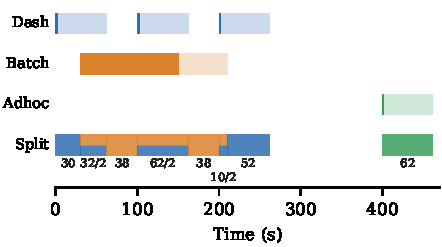
\includegraphics[width=\columnwidth]{figs/example.pdf}
\caption{Worked example, \autos{} 60\,s. Top rows: each team's queries (solid) and tails (light). Bottom row: the Shapley
split; each elementary segment is divided equally among the teams covering it (labels: length / number of teams).}
\label{fig:example}
\end{figure}

\subsection{A worked example}\label{sec:example}
Figure~\ref{fig:example} shows three teams on one warehouse with \autos{} 60\,s: a dashboard team runs three 2-second
queries at 0, 100 and 200\,s; a batch team runs one query from 30 to 150\,s; an ad hoc team runs one 2-second query at
400\,s. The warehouse is billed 324\,s in two periods, of which only 126\,s have a query running. Table~\ref{tab:example}
lists each rule's charges. Proportional splitting charges the batch team 306\,s, far above the 180\,s its own warehouse
would cost, because the remainder follows execution time while the idle tails come from the dashboard team's scattered
queries. Equal and marginal splitting charge the ad hoc team more than its own 62\,s. Shapley charges the ad hoc team exactly
its standalone cost---no one else is up at 400\,s---and splits the first period by who is up when.

\begin{table}[t]
\caption{Charges (billed seconds) in the worked example. Bold: above the team's standalone cost.}\label{tab:example}
\small
\begin{tabular}{lrrrrrr}
\toprule
Team & standalone & R1 & R2 & R3 & R4 & R5 \\
\midrule
Dashboard & 186 & 5   & 12.9 & 108 & 120.8 & 134 \\
Batch     & 180 & 119 & \textbf{306.0} & 108 & 111.9 & 128 \\
Ad hoc    & 62  & 2   & 5.1  & \textbf{108} & \textbf{91.3} & 62 \\
\midrule
Total     & 324 & 126 & 324 & 324 & 324 & 324 \\
\bottomrule
\end{tabular}
\end{table}

\subsection{Fairness properties and the rules we compare}\label{sec:rules}
A chargeback assigns each team $i$ a charge $x_i$. We ask for:
\textbf{(P1) recovery}, $\sum_i x_i$ equals the invoice;
\textbf{(P2) standalone bound}, $\sum_{i \in S} x_i \le c(S)$ for every coalition $S$---no team or group pays more than its
own warehouse would have cost (the core); and
\textbf{(P3) bystander monotonicity}, if one team adds work, no other team's charge rises.
We also look informally at \textbf{responsiveness}: whether the split follows who keeps the warehouse running.
We compare five rules:
\textbf{R1} execution-time attribution (each second with queries running is split equally among them; idle time is left
unassigned---native attribution weights by resource use, which traces do not record);
\textbf{R2} R1 plus the remainder in proportion to R1 (proportional);
\textbf{R3} equal split;
\textbf{R4} leave-one-out marginal cost $c(N) - c(N\setminus\{i\})$, rescaled to the invoice;
\textbf{R5} Shapley (Theorem~\ref{thm:coverage}).

Table~\ref{tab:props} summarises which properties each rule guarantees when $a \ge \mu$. R1 meets P2 trivially because it
assigns only execution time, but fails P1. R2 fails P2 (Table~\ref{tab:example}) and P3: a team that adds one isolated
1-second query raises the bill by 61\,s but its execution share by only 1\,s, so everyone else's proportional charge rises.
R3 fails both, since any growth that raises the bill raises everyone's equal share. R4 fails P2 after rescaling (Table~\ref{tab:example}) and P3. Its
failure of P3 comes from the rescaling alone: another team's growth can only shrink a bystander's raw marginal cost, but it can
shrink the sum of marginals faster, which raises the factor that scales every marginal up to the invoice. R5 meets all three
(Theorem~\ref{thm:coverage}, Proposition~\ref{prop:bystander}). All five rules are cheap: R1, R2 and R5 need one sweep,
$O(m \log m)$; R4 needs $n$ leave-one-out coalition costs, $O(nm)$ after sorting.

\begin{table}[t]
\caption{Properties guaranteed when \autos{} $\ge$ 60\,s.}\label{tab:props}
\small
\begin{tabular}{lccccc}
\toprule
Property & R1 & R2 & R3 & R4 & R5 \\
\midrule
P1 recovery            & \no  & \yes & \yes & \yes & \yes \\
P2 standalone bound    & \yes & \no  & \no  & \no  & \yes \\
P3 bystander monotone  & \yes & \no  & \no  & \no  & \yes \\
\bottomrule
\end{tabular}
\end{table}

\section{Implementation: the Chargeback Engine}\label{sec:impl}
The engine takes a warehouse's query history (team label, execution start and end) and its \autos{}, and produces per-team
charges that sum to the metered invoice. Algorithm~\ref{alg:engine} shows the steps. Coalition costs never touch raw queries
again after step~1, which keeps every rule linear-logarithmic in the number of queries.

\begin{algorithm}[t]
\caption{Chargeback for one warehouse and one billing period}\label{alg:engine}
\small
\begin{algorithmic}[1]
\Require queries $(i, s, e)$; auto-suspend $a$; metered invoice $I$ (seconds)
\State $A_i \gets$ merge $\{[s, e+a]\}$ of team $i$ \Comment{per team, sort + one pass}
\State $B \gets \sum_{C \in \text{comp}(\cup_i A_i)} \max(\mu, |C|)$ \Comment{modelled bill (Lemma~\ref{lem:periods})}
\State \textbf{reconcile:} compare components of $\cup_i A_i$ with the platform's resume/suspend events; flag mismatches
\If{$a \ge \mu$} \State $\phi \gets$ sweep over endpoints of all $A_i$ (Theorem~\ref{thm:coverage}(iii))
\Else \State $\phi \gets$ mean marginal cost over 2,000 random team orders
\EndIf
\State \Return $x_i = \phi_i \cdot I / B$ \Comment{scale to the metered invoice}
\end{algorithmic}
\end{algorithm}

\textbf{One SQL statement.} Because the rule only needs interval merging and a sweep, it can run where the query history
already lives. Figure~\ref{lst:sql} computes $\phi$ in SQL with cumulative window functions only: a gaps-and-islands pass
merges each team's intervals into $A_i$; a running sum over the $\pm1$ endpoint events gives $|N(x)|$ on each elementary
segment; a second running sum gives the prefix $G$; and each team is charged $G(e) - G(s)$ over its components
(Theorem~\ref{thm:coverage}(iii)). There is no range join, so the cost is a few sorts. On 500 random instances, including
ties and zero-length queries, its charges matched the Python sweep to within $2\times10^{-12}$\,s and brute-force Shapley to
within $10^{-12}$\,s. On synthetic months with one million queries, ten teams and exponential run times it took 0.83\,s
($a=600$) and 1.08\,s ($a=60$, with many more components) in DuckDB on one core, and about 0.6\,s on four. We also ran the listing, exactly as printed, inside Snowflake on
the X-Small warehouse of our live run (Section~\ref{sec:method}). Over that run's own query history it matched the Python
sweep to within $3\times10^{-13}$\,s at both settings. On a one-million-row synthetic month generated in Snowflake it took
1.0\,s at $a = 600$ and 3.5\,s at $a = 60$, end to end on the smallest warehouse size.

\begin{figure}[t]
\begin{lstlisting}
WITH iv AS (SELECT team, s, e + :a AS e FROM queries),
ord AS (SELECT team, s, e, MAX(e) OVER (PARTITION BY team
          ORDER BY s, e ROWS BETWEEN UNBOUNDED PRECEDING
          AND CURRENT ROW) AS cm FROM iv),
isl AS (SELECT team, s, e, CASE WHEN s <= LAG(cm) OVER (PARTITION
          BY team ORDER BY s, e) THEN 0 ELSE 1 END AS new FROM ord),
grp AS (SELECT team, s, e, SUM(new) OVER (PARTITION BY team ORDER
          BY s, e ROWS UNBOUNDED PRECEDING) AS k FROM isl),
cover AS (SELECT team, MIN(s) s, MAX(e) e FROM grp GROUP BY team, k),
ev AS (SELECT t, SUM(d) d FROM (SELECT s t, 1 d FROM cover UNION ALL
          SELECT e, -1 FROM cover) x GROUP BY t),
cnt AS (SELECT t, SUM(d) OVER (ORDER BY t ROWS UNBOUNDED PRECEDING)
          n, LEAD(t) OVER (ORDER BY t) t2 FROM ev),
w AS (SELECT t, CASE WHEN n > 0 THEN (t2 - t) / n ELSE 0 END x
          FROM cnt),
g AS (SELECT t, SUM(x) OVER (ORDER BY t ROWS UNBOUNDED PRECEDING)
          - x AS g FROM w)
SELECT c.team, SUM(ge.g - gs.g) AS charge_s FROM cover c
  JOIN g gs ON gs.t = c.s JOIN g ge ON ge.t = c.e GROUP BY c.team;
\end{lstlisting}
\caption{Coverage-Shapley chargeback in SQL (valid for \autos{} $\ge$ 60\,s). Input: \texttt{queries(team, s, e)} for one
warehouse and billing period; output sums to the billed seconds.}
\label{lst:sql}
\end{figure}

\textbf{Correctness and cost.} The engine is under 200 lines of Python plus tests. On 1,600 random instance--setting pairs
with $a \ge 60$\,s the sweep matched brute-force Shapley to within $3\times10^{-13}$\,s and recovered the bill exactly; on 300
further instances no coalition was charged above its standalone cost. On a synthetic month with one million queries and ten
teams, the Python sweep takes 0.2--1.2\,s depending on the machine and all five rules, including $n$ leave-one-out coalition costs for R4, 6.7--7.3\,s
on one core. The full Redset study (94 instances, four settings, three months) ran on a laptop.

\textbf{Reconciliation.} The modelled bill $B$ and the metered invoice $I$ differ for reasons outside the model: cloud-services
credits, statements that run without the warehouse, and the platform's suspend lag. The engine therefore first checks that
the modelled running periods match the platform's resume and suspend events, and only then scales every charge by $I/B$.
For a given invoice, scaling by a constant preserves P1 and P2 relative to scaled standalone costs; P3 holds for the model
charges, and for scaled charges only while $I/B$ stays fixed.

\section{Methodology}\label{sec:method}
\textbf{Pre-registration.} The inclusion rule, interval definition, settings, rules and metrics were written and timestamped
before any result was computed; later additions (implementation choices, the definition of ``doubling'') were added as dated
addenda before the corresponding runs. Two deviations are disclosed.
(1)~The first full run summed raw execution seconds for R1, which double-counts concurrent queries and produced impossible
negative ``unassigned'' shares. We fixed R1 to split concurrent seconds, re-ran everything, kept the first output, and report
only the re-run; R3--R5, standalone costs and coalition costs are unaffected by the fix.
(2)~An independent re-computation of every number in this paper, done after all runs, found that the runner cut calendar
months in the analyst's local time zone. Redset starts at midnight UTC on March 1, so its first five hours formed a
``February'' stub month (56 instance-months per setting, median 5.2 billed hours against about 600 for full months). We drop
the stub, as the frozen definition (calendar months, March--May) intended, and report results with it kept in
Section~\ref{sec:sens}. Month boundaries remain those of US Eastern time (4--5 hours from UTC), and the first five hours of
data are dropped rather than moved into March. The fleet headlines move by less than three points; month-to-month stability
and the tail-intensity analysis move more, and we report both ways. Results marked \emph{exploratory} were not pre-registered.

\textbf{Redset.} Redset~\cite{redset} releases three months (March--May 2024) of query metadata for 200 provisioned and 200
serverless Redshift instances, with user, arrival, queue, compile and execution times. A team is a user within an instance.
An instance is included if at least two teams each account for at least 1\% of its execution time over at least seven days:
95 of 400 instances qualify (233 have a single user), holding 247.8 million queries; 94 have at least one month with two
active teams. Teams below 1\% are pooled into ``other'', which is charged but not reported. A query occupies
$[\text{arrival} + \text{queue},\ \text{arrival} + \text{queue} + \text{compile} + \text{execution}]$; result-cache hits with
no execution are dropped. Each instance is replayed as a counterfactual per-second warehouse of fixed size under \autos{} 60,
300 and 600\,s (and 30\,s, reported separately), per calendar month: 264 instance-months and 1,414 team-months per setting.
Redshift's own billing differs (provisioned clusters bill by node-hour); we use its workloads, not its prices.

\textbf{Metrics.} For P2 we check every coalition when a month has at most ten teams, and otherwise all singletons, pairs
and leave-one-out complements: 25,856 coalitions per setting. For P3 we take each instance-month and each team in turn,
double that team (a copy of each query starting when the original ends), and record whether any other team's charge rises:
7,096 bystander cases per setting. Doubling in place adds at most as much bill as execution time, so R2 passes this test by
construction. A second, pre-registered before it was run, exercises R2: each team in turn adds ten one-second queries at
random times in the month, the kind of growth that adds tails rather than execution (7,096 cases per setting). For responsiveness we measure how much each team's share
of the bill moves when \autos{} changes from 60 to 600\,s; for stability, the month-to-month variation of charges for teams
whose own usage varied by less than 10\%.

\textbf{Snowflake run.} This run is separate from any other study's; it was designed and run for this paper only. On a dedicated Gen2 X-Small warehouse with query acceleration disabled, four tagged teams ran seeded
schedules for 60 minutes at \autos{} 60\,s and 60 minutes at 300\,s: a dashboard team (bursts of five queries every 3--5
minutes), a batch team (one join every 15 minutes), an ad hoc team (Poisson, mean gap six minutes) and a trickle team (a
point query every two minutes); result cache off; 236 statements, all successful. Ground truth comes from Snowflake's
\texttt{QUERY\_HISTORY}, \texttt{QUERY\_ATTRIBUTION\_HISTORY}, \texttt{WAREHOUSE\_EVENTS\_HISTORY} and
\texttt{WAREHOUSE\_METERING\_HISTORY}. The 300\,s phase was disrupted: the client machine slept, and its statements spread
over about 2.5 hours instead of one. The validation below uses what actually ran and is unaffected; the planned timing was
not.

\section{Results}
\subsection{Does the billing model match Snowflake?}\label{sec:e1}
Table~\ref{tab:e1} compares the model's running periods, derived from \texttt{QUERY\_HISTORY} execution intervals, with
the warehouse's actual resume and suspend events. The model reproduces every running period and 98.9\% (60\,s) and 99.5\%
(300\,s) of the running time between resume and suspend events. The warehouse suspended a median 60.1\,s and 300.3\,s after its last query, within 0.4\,s of
the setting; we did not observe the up-to-30-second lag the documentation allows. Assumption A2 therefore held to within a
fraction of a second on this account. The metered compute was 0.953 and 1.426 credits for the two phases, or
1.34--1.35 credits per hour of running time.

\begin{table}[t]
\caption{Modelled running periods vs.\ Snowflake's resume and suspend events (live four-team run).}\label{tab:e1}
\small
\begin{tabular}{lrrrrr}
\toprule
\autos & periods (m/a) & model s & actual s & ratio & tail \\
\midrule
60\,s  & 30 / 30 & 2{,}512 & 2{,}541 & 0.989 & 60.1\,s \\
300\,s & 3 / 3   & 3{,}799 & 3{,}820 & 0.995 & 300.3\,s \\
\bottomrule
\end{tabular}
\end{table}

\subsection{How much of the bill is unassigned?}\label{sec:e2}
Figure~\ref{fig:e2} shows, per Redset instance, the share of the bill that execution-time attribution leaves unassigned.
The median is 31.4\% at 60\,s, 50.2\% at 300\,s and 56.3\% at 600\,s; the interquartile range at 600\,s is 17--78\%.
The 19 serverless instances leave more unassigned (median 73.3\% at 600\,s) than the 75 provisioned ones (47.1\%). In the live run, Snowflake's own attribution assigned 0.118 of 0.953 metered credits at 60\,s and 0.104 of
1.426 at 300\,s: 87.7\% and 92.7\% unassigned. Snowflake attributed six (60\,s) to eleven (300\,s) times more than pure
execution seconds on these short queries---native attribution evidently counts more than execution---so the Redset figures
are best read as what execution-time accounting leaves over. On our one live run, the platform's own attribution assigned
more, yet still left most of the bill unassigned.
Either way, the remainder is the larger part of the bill for most instances, and the rule that splits it decides most of
what each team pays.

\begin{figure}[t]
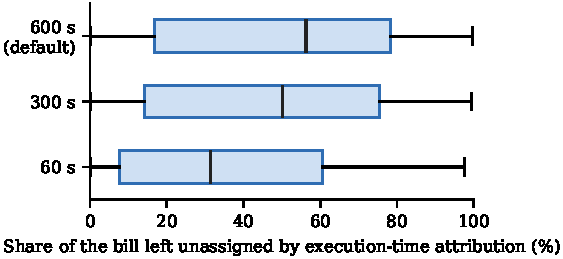
\includegraphics[width=\columnwidth]{figs/e2_unassigned.pdf}
\caption{Share of each Redset instance's bill (94 instances, three months) left unassigned by execution-time attribution.}
\label{fig:e2}
\end{figure}

\subsection{Are the common rules fair?}\label{sec:e3}
\textbf{Standalone bound (P2).} Figure~\ref{fig:e3} and Table~\ref{tab:e3} report how often each rule charges a team, or a
group of teams, more than its own warehouse would have cost. Proportional splitting does so for 12--17\% of team-months and
8--11\% of coalitions; equal splitting for 33--44\% of team-months; leave-one-out marginal cost for 3--4\%. The Shapley
rule never does: zero of 1,414 team-months and zero of 25,856 coalitions at each setting, as Theorem~\ref{thm:coverage}
predicts. These rates include the pooled ``other'' team; for the 1,187 named team-months alone they are 15--18\% for
proportional, 29--40\% for equal and 3--4\% for marginal splitting. The rules also disagree about who pays: the share of the
fleet's bill that moves between teams relative to Shapley has a median of 16--27\% for proportional, 37--42\% for equal and
6--18\% for marginal splitting. The overcharges are not marginal. A team that proportional splitting overcharges pays a median 33--44\% more than
its standalone cost, and one in ten pays about three times as much (exploratory); a team that equal splitting overcharges
pays a median 2.6--3.2 times its standalone cost. Marginal splitting's overcharges are small (median 2--3\%), but it fails the bystander test below.

The live run shows the same failures with real metering. At 60\,s proportional splitting charged the dashboard team 0.543
credits against a standalone cost of 0.383, and the batch team 0.143 against 0.094; at 300\,s marginal splitting charged the
ad hoc team 0.790 against 0.768. Shapley charged every team less than its standalone cost in both phases (Table~\ref{tab:live}). The pre-registered criterion for a primary claim---it must hold on Redset and match in direction on the Snowflake
run---is met for both: the common rules exceed standalone costs in both, and Shapley stays within them in both.

\begin{table}[t]
\caption{Live run: per-team charges (credits), scaled to the metered invoice. Alone: standalone cost; bold: above it.}\label{tab:live}
\small
\setlength{\tabcolsep}{3pt}
\begin{tabular}{llrrrrr}
\toprule
\autos & Team & alone & R2 & R3 & R4 & R5 \\
\midrule
60\,s  & dashboard & 0.383 & \textbf{0.543} & 0.238 & 0.208 & 0.252 \\
       & trickle   & 0.686 & 0.148 & 0.238 & 0.559 & 0.514 \\
       & batch     & 0.094 & \textbf{0.143} & \textbf{0.238} & 0.054 & 0.058 \\
       & ad hoc    & 0.189 & 0.119 & \textbf{0.238} & 0.133 & 0.130 \\
\midrule
300\,s & dashboard & 1.272 & 0.833 & 0.357 & 0.354 & 0.505 \\
       & trickle   & 1.262 & 0.102 & 0.357 & 0.282 & 0.495 \\
       & batch     & 0.453 & 0.374 & 0.357 & 0.000 & 0.123 \\
       & ad hoc    & 0.768 & 0.117 & 0.357 & \textbf{0.790} & 0.303 \\
\bottomrule
\end{tabular}
\end{table}

\begin{figure}[t]
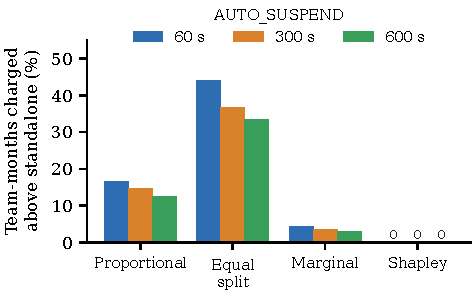
\includegraphics[width=\columnwidth]{figs/e3_overcharge.pdf}
\caption{Team-months charged above their standalone cost, by rule and auto-suspend setting (1,414 team-months).}
\label{fig:e3}
\end{figure}

\begin{table}[t]
\caption{Standalone-bound violations: team-months / coalitions charged above standalone cost.}\label{tab:e3}
\small
\begin{tabular}{lccc}
\toprule
Rule & 60\,s & 300\,s & 600\,s \\
\midrule
R2 proportional & 16.6\% / 10.7\% & 14.7\% / 8.7\% & 12.4\% / 7.6\% \\
R3 equal split  & 44.1\% / 20.8\% & 36.6\% / 15.0\% & 33.4\% / 12.8\% \\
R4 marginal     & 4.3\% / 2.1\%   & 3.5\% / 1.4\%   & 3.0\% / 1.6\% \\
R5 Shapley      & 0 / 0           & 0 / 0           & 0 / 0 \\
\bottomrule
\end{tabular}
\end{table}

\textbf{Bystander monotonicity (P3).} Figure~\ref{fig:e4} shows both growth tests. When one team doubles its work,
marginal-cost splitting raised another team's charge in 42.3\% of 7,096 cases at 60\,s and 31.1\% at 600\,s (median rise
0.8\% and 0.5\%); proportional splitting cannot fail this test. When one team instead adds ten isolated one-second queries,
proportional splitting raised another team's charge in 67.9\% of cases at 60\,s and 40.6\% at 600\,s, and marginal splitting
in 50.2\% and 26.2\%. The rises are small (medians of 0.01--0.2\% of the bystander's charge), because ten queries in a month
is small growth; what matters is the direction---a team is billed more because someone else changed their behaviour.
Shapley never raised a bystander's charge in either test, 14,192 cases per setting in all, matching
Proposition~\ref{prop:bystander} and the expectation stated before the runs.

\begin{figure}[t]
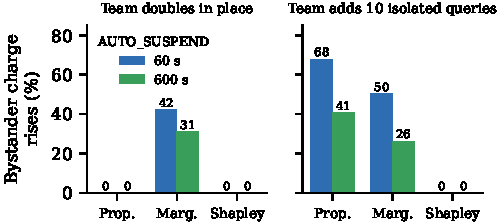
\includegraphics[width=\columnwidth]{figs/e4_bystander.pdf}
\caption{Share of cases in which another team's charge rises when one team grows: doubling its work in place (left) or
adding ten isolated one-second queries (right); 7,096 cases per test and setting.}
\label{fig:e4}
\end{figure}

\subsection{Who pays more under a fair rule?}\label{sec:who}
\textbf{Responsiveness.} Proportional splitting is, by construction, blind to who keeps the warehouse up: when the setting
changes from 60 to 600\,s, a team's share of the bill moves by a median 0.0 percentage points. The Shapley share moves by a
median 2.3 points (90th percentile 13.1) toward the teams whose activity or tails keep the warehouse running; marginal shares
move erratically (median 1.5, 90th percentile 22.4).

\textbf{Tail intensity} (exploratory). Figure~\ref{fig:who} orders teams by the ratio of their standalone cost to their
execution time, a measure of how much idle tail each second of work brings with it. Teams in the lowest decile by rank (ratio below
1.3--1.9, mostly long-running work) pay a median 7.5 (60\,s), 12.5 (300\,s) and 16.3 (600\,s) percentage points less of the
bill under Shapley than under proportional splitting; teams in the highest decile (ratio above 12--39: short, scattered
queries such as dashboards and probes) pay 6.8, 10.9 and 8.4 points more. With the stub months kept, the lowest decile
at 600\,s pays 19.8 points less; the direction holds in every setting. This is the mechanism behind proportional overcharges: a team with long
queries but few resumes pays for idle tails that other teams cause. For a platform team, it also predicts who will object
to a switch, and why.

\begin{figure}[t]
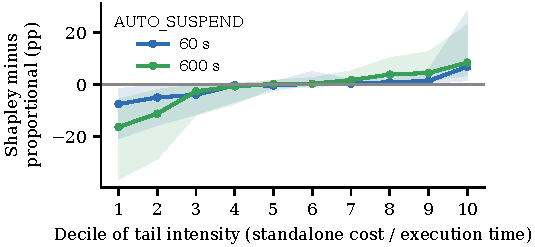
\includegraphics[width=\columnwidth]{figs/who_pays.pdf}
\caption{Shapley share minus proportional share by decile of tail intensity (median and interquartile band; 1,187 named
team-months per setting). Exploratory.}
\label{fig:who}
\end{figure}

\textbf{How far the rules move each team.} Figure~\ref{fig:gap} shows, for every named team-month, how many percentage
points of the bill each rule moves away from the Shapley share. At 600\,s the median team moves 4.7 points under
proportional, 9.2 under equal and 3.6 under marginal splitting, and 32\%, 46\% and 28\% of team-months move by more than
ten points. These are not rounding differences: a tenth of the teams see a fifth or more of the bill change hands.

\begin{figure}[t]
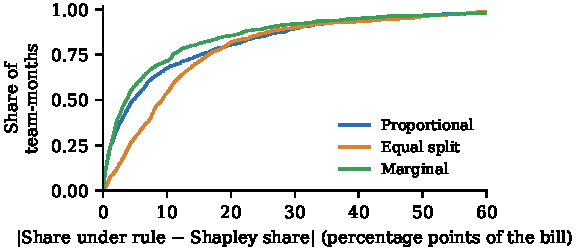
\includegraphics[width=\columnwidth]{figs/share_gap.pdf}
\caption{Distribution, over 1,187 named team-months at 600\,s, of the absolute difference between each rule's share of the
bill and the Shapley share. Exploratory.}
\label{fig:gap}
\end{figure}

\textbf{Stability.} For the 117 teams whose own monthly usage varied by less than 10\%, the coefficient of variation of the
monthly charge is 3.8--4.5\% under Shapley, 5.6--5.9\% under proportional splitting and 9.0--26.6\% under marginal splitting.
Of these teams, 115 have all three months. On this data the fair rule is
also the steadiest, but the margin is small and not robust: with the stub month kept, only 29 teams qualify and Shapley and
proportional are indistinguishable (4.3--5.0\% against 4.1--6.1\%). Stable usage here means a coefficient of variation of
monthly execution seconds below 10\%.

\subsection{A case study}\label{sec:case}
Table~\ref{tab:case} shows one Redset instance, chosen as the one with the largest proportional overcharge among instances
with four to six named teams; we show it because the pattern is stable across its three months, not because it is typical.
Team~1 runs only 0.5\% of the execution time, but its queries are spread so evenly that it alone would keep the warehouse
up for the entire month: its standalone cost equals the whole bill. Team~2 does most of the work in a few hundred hours.
Proportional splitting follows execution and charges team~2 81\% of the bill, 4.2 times what its own warehouse would cost;
team~1 pays 2.5\%. Marginal splitting goes to the other extreme: removing any other team saves nothing, so every
marginal is zero except team~1's, and team~1 pays the whole bill. Shapley charges team~1 71\% for the tails only it causes
and splits the shared hours, leaving team~2 at 8\%, below its standalone cost; every other team is also below its own.
The same ordering holds in April and May (team~2 under proportional: 3.9 and 3.3 times its standalone cost) and at
60\,s (2.8--3.4 times). A platform team that sees this table knows what to do next: the expensive behaviour is team~1's
keep-alive pattern, not team~2's heavy queries.

\begin{table}[t]
\caption{Case study: Redset instance provisioned/106, March 2024, \autos{} 600\,s. Execution and charges as \% of the
743-hour bill; alone = standalone cost in hours. Bold: above standalone cost.}\label{tab:case}
\small
\setlength{\tabcolsep}{3.5pt}
\begin{tabular}{lrrrrrr}
\toprule
Team & exec. & alone & R2 & R3 & R4 & R5 \\
\midrule
1       & 0.5 & 743\,h & 2.5  & 20.0 & 100.0 & 70.9 \\
2       & 17.5 & 143\,h & \textbf{81.0} & \textbf{20.0} & 0.0 & 8.0 \\
3       & 2.2 & 140\,h & 10.1 & \textbf{20.0} & 0.0 & 8.2 \\
0       & 1.2 & 208\,h & 5.5  & 20.0 & 0.0 & 12.3 \\
other   & 0.2 & 14\,h  & 0.8  & \textbf{20.0} & 0.0 & 0.6 \\
\bottomrule
\end{tabular}
\end{table}

\subsection{Below the minimum and sensitivity}\label{sec:sens}
At \autos{} 30\,s the minimum can bind and R5 is sampled. It violated the standalone bound in 1 of 25,856 coalition checks
and for no team-month, against 17.5\% of team-months for proportional and 45.8\% for equal splitting; the median unassigned
share is 27.5\%. Proposition~\ref{prop:below} shows the core guarantee does not carry over; in practice the gap was
negligible on this fleet.

How accurate is the sampled path? On 300 random instances with four to eight teams, $a \in \{0, 30\}$\,s and short queries
over an hour, so that the minimum binds often, we computed the exact Shapley value by brute force (exploratory;
Table~\ref{tab:sampled}). With 2,000 sampled orders the largest per-team error was a median 0.07\% of the bill (95th
percentile 0.27\%); quadrupling the orders roughly halves it, as sampling theory predicts. Neither the exact nor the sampled
values violated the standalone bound in any of 30,472 coalition checks. Simply applying the sweep, rescaled to the bill,
is not a usable shortcut: its error was a median 5\% of the bill, and it violated the standalone bound in 246 of the 300
instances.

\begin{table}[t]
\caption{Sampled Shapley below the minimum vs.\ exact (300 random instances): largest per-team error, \% of the bill.}\label{tab:sampled}
\small
\begin{tabular}{lrrr}
\toprule
Method & median & 95th pct. & max \\
\midrule
100 orders   & 0.33 & 1.27 & 2.75 \\
500 orders   & 0.14 & 0.55 & 0.85 \\
2,000 orders & 0.07 & 0.27 & 0.60 \\
5,000 orders & 0.05 & 0.18 & 0.41 \\
Sweep, rescaled & 5.01 & 17.68 & 28.41 \\
\bottomrule
\end{tabular}
\end{table}
 Keeping the five-hour stub months (320 instance-months, 1,653 team-months, 29,262 coalitions,
7,938 bystander cases per setting) changes the unassigned medians by at most 0.1 points, the overcharge rates by at most
1.1, the doubling-test rates for marginal splitting to 40.0\% and 28.4\%, and the isolated-query rates to 64.3\% and 37.3\%
(proportional) and 47.8\% and 24.4\% (marginal); Shapley still has zero violations of any kind.

\textbf{What if teams would run faster alone?} Assumption A1 keeps every query's timing when other teams are removed. With
less contention a team alone might run faster, which lowers its standalone cost. A pre-registered run (Addendum~5) shortened
every query of each named team by 10, 20 and 30\% when computing its standalone cost, while keeping the charges computed at
observed timing. Our stated expectation, that Shapley would stay at or near zero violations at 10\%, was wrong. At 10\%,
Shapley charged 8.5\% of named team-months above the shortened standalone cost at 60\,s and 3.1\% at 600\,s, by a median of
2.1\% and 0.4\% (90th percentile 8.1\% and 3.6\%); at 30\%, 14.4\% and 4.6\%. The violators are mostly teams that already
pay exactly their standalone cost---about two thirds had less than 1\% slack at observed timing---because they run almost
alone. For those teams, there is little contention to remove, so a uniform speed-up overstates the effect. The common rules
do worse under the same test. At 10\%, proportional splitting exceeds the shortened standalone cost for 21.1\% (60\,s) and
15.4\% (600\,s) of team-months, by a median 31\% and 42\%; equal splitting for 40.4\% and 29.1\%, by a median 164\% and
121\%; and marginal splitting for 13.9\% and 8.8\%, by a median 2.5\% and 0.6\%. The standalone guarantee is therefore exact under A1 and approximate beyond it, and Shapley's violations are the
fewest or smallest at every speed-up tested.

\section{Deployment Lessons}\label{sec:lessons}
\textbf{Reconcile before you allocate.} The engine first reproduces the warehouse's running periods from query history and
compares them with the platform's resume and suspend events; only then does it split the metered invoice. A mismatch signals
untagged work on the warehouse---an administrator's session, a scheduled task, a BI tool's keep-alive---which should be found
before any team is charged.

\textbf{Labels belong to the platform.} Chargeback is only as good as the team label. Session-level query tags were complete
in our run. Proposition~\ref{prop:labels} adds a reason beyond hygiene: under Shapley, two teams can lower their joint
charge by sharing a label, so labels should come from the service account or role that submits the query, not from a tag a
team sets itself.

\textbf{Publish the rule, and start with showback.} The coverage interpretation---``each billed second is shared by the
teams keeping the warehouse up''---is easy to explain to finance and to the teams, which matters as much as the axioms.
Section~\ref{sec:who} predicts the objection: teams with short, scattered queries will see their share rise. Publishing both
charges side by side for a quarter before money moves lets teams see why, and the per-segment breakdown answers a dispute
with the seconds in question.

\textbf{Use the sampled path below 60\,s.} Below 60\,s the minimum binds and the exact sweep no longer applies; sampling
with 2,000 orders was within the standalone bound in all but one of 25,856 fleet checks and within 0.3\% of the exact value
in 95\% of random instances (Table~\ref{tab:sampled}). Use a fixed seed so that a month's charges can be reproduced.

\textbf{Run it monthly, where the data lives.} The SQL version runs inside the warehouse over the platform's own query
history in seconds, so the chargeback can be recomputed for every billing period and for every warehouse without moving
data. Keeping each month's per-segment output makes the charge auditable: any team can see which seconds it paid for and
with whom it shared them.

\textbf{Expect a few large movers.} Most teams' shares move by a few points when the rule changes, but between a quarter and
half move by more than ten (Figure~\ref{fig:gap}). Those teams---often a keep-alive or polling pattern, as in Table~\ref{tab:case}---are
where the conversation with finance and with the team will happen, and where a change in behaviour saves the most.

\textbf{Chargeback changes behaviour.} A rule that charges for tails gives teams a reason to batch scattered queries or move
them to a smaller warehouse---the behaviour a platform wants. A rule that hides tails in a proportional remainder rewards
the opposite.

\section{Beyond Snowflake}\label{sec:beyond}
The game depends only on the billing contract, and the contracts of other services share its parts. Databricks SQL
warehouses accrue charges while idle until an auto-stop timeout stops them---at least ten minutes for pro and classic
warehouses, and down to one minute for serverless ones set through the API~\cite{dbx-warehouse}: the same tail structure, so Theorem~\ref{thm:coverage} applies whenever the timeout is at
least any start-up minimum. Redshift Serverless bills RPU-seconds with a 60-second minimum but does not bill idle
time~\cite{rs-serverless}; that is our model with $a = 0 < \mu$, the case of Proposition~\ref{prop:below}, so the sampled path
applies. BigQuery bills autoscaled slots per second with a one-minute minimum and retains scaled capacity for at least 60
seconds~\cite{bq-autoscale}, which plays the role of $a = \mu = 60$\,s for the on/off part of a shared reservation; sharing
the bill for how \emph{much} capacity runs, rather than \emph{whether} it runs, is a different game that we leave open.

\section{Limitations}
Redset workloads are replayed under per-second billing at a fixed size; we use their timing, not Redshift's prices. Users
stand in for teams. A1 assumes that removing teams does not change the remaining queries' timing; under heavy contention a
smaller coalition would run faster. Section~\ref{sec:sens} shows that a uniform 10\% speed-up breaks the standalone bound
for 3--9\% of team-months, by a median 0.4--2\%; a contention-aware model of standalone runtimes is future work. R1 approximates native attribution by an
equal split of concurrent seconds, and Snowflake's attribution assigned more than this on short queries. The live run is a
single warehouse on one trial account over two hours, one phase of which was disrupted; it validates the billing model, not
the fleet-level percentages. The tail-intensity analysis is exploratory. Multi-cluster warehouses, mid-period resizing and
cloud-services credits are out of scope.

\section{Future Work}
Exact or bounded allocations for \autos{} below 60\,s; allocation under multi-cluster scaling, where the number of running
clusters is itself shared; chargeback that includes cloud-services and serverless features; and a field study of how teams
respond to a published rule.

\section{Artifacts}\label{sec:artifacts}
Code, raw results, the Snowflake run logs and Snowflake's own records for the live run, and the pre-registration with every
dated addendum and deviation are at \url{https://github.com/khadarvalishaik0520/shared-warehouse-chargeback}. One command
(\texttt{./run.sh analysis}) regenerates every number, table and figure in this paper from the committed result files in
minutes, without downloading Redset; re-running the replays needs Redset and takes hours. Unit tests check the sweep
against brute-force Shapley and the SQL against the sweep.

\section{Conclusion}
The idle part of a shared warehouse's bill is large---a median of a third to more than half under execution-time
accounting---and the rules used to split it are not fair: proportional, equal and marginal splitting overcharge teams
relative to their own warehouse or penalise bystanders. Because per-second billing with an idle timeout is a coverage game
whenever the timeout is at least the resume minimum, the Shapley chargeback is both principled and cheap: split each billed
second among the teams keeping the warehouse up. It fits in one SQL statement and, at observed timing, never exceeded any team's or group's
standalone cost, never charged a bystander for someone else's growth, and reconciles to the invoice.

\begin{acks}
AI-generated content: Claude (Anthropic) was used to draft and edit the text (all sections), to write the engine, analysis
code and SQL listing (Sections~\ref{sec:impl}--\ref{sec:sens}), and to produce the figures and tables. The author directed the study and ran the
experiments; every reported number was re-computed from the result files, and the author takes full responsibility for
the content.
\end{acks}

\bibliographystyle{ACM-Reference-Format}
\bibliography{refs}
\end{document}
